\section{실험}
\label{sec:experiments}

우리는 표준 mathematical reasoning 및 coding benchmarks에서 JustGRPO를 평가한다. 우리의 실험 설계는 두 가지 가설을 검토하는 것을 목표로 한다. (i) RL training 동안 autoregressive (AR) order를 강제하면 복잡한 arbitrary-order approximation에 의존하지 않고도 reasoning capabilities를 효과적으로 끌어낼 수 있다는 점, (ii) 이 제약은 최적화 objective에만 적용되어 inference 시 diffusion model의 parallel decoding capabilities는 그대로 유지된다는 점이다.

\begin{table}[t]
    \centering
    \caption{LLaDA-Instruct에서 post-training approaches의 \textbf{system-level comparison}. JustGRPO는 단순함에도 강한 성능을 달성한다.
    Baseline 수치는 대부분 각 원 논문에서 인용했다\protect\footnotemark{}.
    이러한 baselines 사이에서 실험 설정이 완전히 일관되지는 않음을 밝혀 둔다. JustGRPO는 모든 tasks에서 full fine-tuning을 사용하고 step마다 하나의 token을 unmask한다. Baseline 중 LLaDA-1.5, LLaDOU, ESPO도 step마다 하나의 token을 unmask하는 반면, 나머지는 step마다 두 개의 token을 unmask한다. LLaDA-1.5와 LLaDOU도 full fine-tuning을 사용하고, ESPO는 code tasks에서만 그렇게 하며(그 외에는 LoRA), 나머지는 LoRA를 사용한다.
    이러한 이질성을 고려하여, 원래 설정이 우리와 다른 몇 가지 대표 baseline을 Table~\ref{tab:controlled_comparison}에서 통일된 protocol 아래 추가로 재현했으며, 여기에서도 동일한 결론이 유지된다.
    \label{tab:main_results}}
    \vskip -.05in
    \renewcommand{\arraystretch}{1.08}
    \resizebox{\linewidth}{!}{
        \begin{tabular}{l ccc ccc ccc ccc}
            \toprule
            & \multicolumn{3}{c}{\textbf{GSM8K}}
            & \multicolumn{3}{c}{\textbf{MATH-500}}
            & \multicolumn{3}{c}{\textbf{HumanEval}}
            & \multicolumn{3}{c}{\textbf{MBPP}} \\
            \cmidrule(lr){2-4}
            \cmidrule(lr){5-7}
            \cmidrule(lr){8-10}
            \cmidrule(lr){11-13}
            \textbf{Model / Seq Len }
            & \textbf{128} & \textbf{256} & \textbf{512}
            & \textbf{128} & \textbf{256} & \textbf{512}
            & \textbf{128} & \textbf{256} & \textbf{512}
            & \textbf{128} & \textbf{256} & \textbf{512} \\
            \midrule
            d1~\cite{zhao2025d1}
            & 73.2 & 81.1 & 82.1
            & 33.8 & 38.6 & 40.2
            & - & - & -
            & - & - & - \\
            LLaDOU$^\dagger$~\cite{huang2025reinforcing}
            & - & 88.1 & -
            & - & 41.1 & -
            & - & \textbf{59.1} & -
            & - & 51.6 & - \\
            LLaDA-1.5$^\ddagger$~\cite{zhu2025llada}
            & - & 83.3 & -
            & - & - & -
            & 29.3 & 39.6 & \textbf{51.9}
            & 39.6 & 39.9 & 38.8 \\
            wd1~\cite{tang2025wd1}
            & 77.2 & 80.8 & 82.3
            & 33.3 & 34.4 & 39.0
            & - & - & -
            & - & - & - \\
            $d$-TreeRPO~\cite{pan2025d}
            & - & 81.2 & 82.6
            & - & 37.7 & 38.9
            & - & - & -
            & - & - & - \\
            ESPO~\cite{ou2025principled}
            & 80.0 & 82.3 & 83.7
            & 36.0 & 39.0 & 43.4
            & 28.1 & 42.1 & 50.0
            & 47.4 & 44.6 & 44.2 \\
            GDPO~\cite{rojas2025improving}
            & 78.4 & 82.8 & 84.5
            & 33.2 & 39.6 & 41.4
            & 26.2 & 39.6 & 39.0
            & 43.6 & 50.6 & 47.1 \\
            SPG~\cite{wang2025spg}
            & 78.5 & 86.1 & 84.5
            & 33.4 & 40.0 & 41.8
            & - & - & -
            & - & - & - \\
            \midrule
            \textbf{JustGRPO}
            & \textbf{83.8} & \textbf{89.1} & \textbf{89.8}
            & \textbf{39.0} & \textbf{45.1} & \textbf{45.2}
            & \textbf{37.8} & 49.4 & 48.7
            & \textbf{50.6} & \textbf{52.4} & \textbf{49.0} \\
            \bottomrule
        \end{tabular}
    }
    \par\vskip 2pt
    \noindent\parbox{\linewidth}{\footnotesize\raggedright
        $^\dagger$ LLaDOU는 auxiliary module로 base architecture를 수정한다.\\
        $^\ddagger$ LLaDA-1.5는 훨씬 더 큰 규모의 비공개 수집 dataset에서 학습된다.}
    \vskip -.05in
\end{table}

\footnotetext{두 가지 예외가 있다. LLaDOU의 MATH-500 결과($41.1$)는 원 논문이 MATH-500이 아니라 전체 MATH test set을 보고하기 때문에 우리가 official checkpoint로 측정했다. LLaDA-1.5 수치는~\cite{ou2025principled}에서 가져왔다.}

\paragraph{실험 설정.}
우리는 LLaDA-Instruct~\cite{nie2025large}에 JustGRPO를 적용하고, 네 가지 표준 reasoning 및 coding benchmarks인 GSM8K, MATH-500, HumanEval, MBPP에서 그 효과를 평가한다.
Mathematical tasks의 경우~\cite{zhao2025d1,ou2025principled}를 따라 각 dataset의 official training split으로 학습한다. Coding tasks의 경우 AceCoder-87K~\cite{zeng2025acecoder}의 subset으로~\cite{gong2025diffucoder,ou2025principled}를 따라 학습한다.
우리는 추가 task-specific SFT 없이 full-parameter fine-tuning을 사용해 JustGRPO를 모델에 직접 적용한다.
우리의 training recipe는 대체로~\cite{huang2025reinforcing}를 따른다.
학습된 모델을 평가하기 위해 표준 LLaDA evaluation protocol~\cite{nie2025large}을 따르며, 이는 32-token block에서 semi-autoregressive decoding과 함께 low-confidence remasking을 적용한다(step마다 하나의 token을 unmask, \ie, generation length 256의 경우 256 steps). Sampling temperature는 0을 사용한다.
우리는~\cite{zhao2025d1,ou2025principled}를 따라 generation length 128, 256, 512에서 모든 benchmarks를 평가한다.
Training에 대한 자세한 내용은 Appendix~\ref{app:experimental_setups}에 제공된다.

\subsection{주요 결과}
\label{subsec:main_results}

\paragraph{Reasoning tasks에서의 성능.} Table~\ref{tab:main_results}는 system-level comparison을 보고한다. 우리는 diffusion-specific RL adaptation이 전혀 필요 없음에도 표준 GRPO 정식화를 단순히 적용하는 것만으로 이미 강한 전반적 성능을 달성함을 관찰한다. GSM8K에서 JustGRPO는 89.1\% accuracy(seq len 256)에 도달하여 이전 diffusion-specific methods와 경쟁적이거나 더 높으며, 더 어려운 MATH-500에서도 유사한 경향을 보인다. 또한 auxiliary trainable module이나 더 큰 규모의 private training data를 활용하고 HumanEval에서 더 높은 accuracy를 보고하는 LLaDOU 및 LLaDA-1.5와도 전반적으로 경쟁력을 유지한다.
\begin{wraptable}{r}{0.58\textwidth}
    \centering
    \vskip -0.15in
    \caption{\textbf{우리 설정과 정렬된 configurations에서의 재현} (full fine-tuning, decoding step마다 하나의 token, generation length 256). 재현한 baselines는 $^{*}$로 표시했다. HumanEval 및 MBPP의 ESPO$^{*}$ 결과는 원 논문에서 직접 가져왔으며, 해당 설정은 이미 우리와 일치한다(full fine-tuning, decoding step마다 하나의 token).}
    \vskip -0.12in
    \label{tab:controlled_comparison}
    \small
    \setlength{\tabcolsep}{4pt}
    \begin{tabular}{lcccc}
        \toprule
        \textbf{Model} & \textbf{GSM8K} & \textbf{MATH-500} & \textbf{HumanEval} & \textbf{MBPP} \\
        \midrule
        d1$^{*}$           & 83.8 & 39.2 & -- & -- \\
        ESPO$^{*}$         & 84.7 & 40.3 & 42.1 & 44.6 \\
        SPG$^{*}$          & 86.9 & 41.8 & -- & -- \\
        \textbf{JustGRPO}  & \textbf{89.1} & \textbf{45.1} & \textbf{49.4} & \textbf{52.4} \\
        \bottomrule
    \end{tabular}
    \vskip -0.12in
\end{wraptable}
Table~\ref{tab:main_results}의 수치는 이질적인 설정에서 paper-reported된 것이므로(캡션 참조), 우리는 우리와 정렬된 통일 protocol(full-parameter fine-tuning, decoding step마다 하나의 token, generation length 256) 아래 대표 baseline들을 추가로 재현한다.
Table~\ref{tab:controlled_comparison}에 보이듯, JustGRPO는 이 비교에서도 여전히 앞서며, 이는 denoising trajectories의 전체 조합 공간 위에서 최적화하는 것이 반드시 필요하지 않을 수 있고, training 동안 dLLM을 sequential generator로 취급하는 것이 일반 reasoning tasks에 단순하지만 효과적인 recipe라는 관점과 일치한다.

\subsection{JustGRPO는 Parallel Decoding을 보존한다}
\label{subsec:parallel_decoding}

\begin{figure}[t]
    \centering
    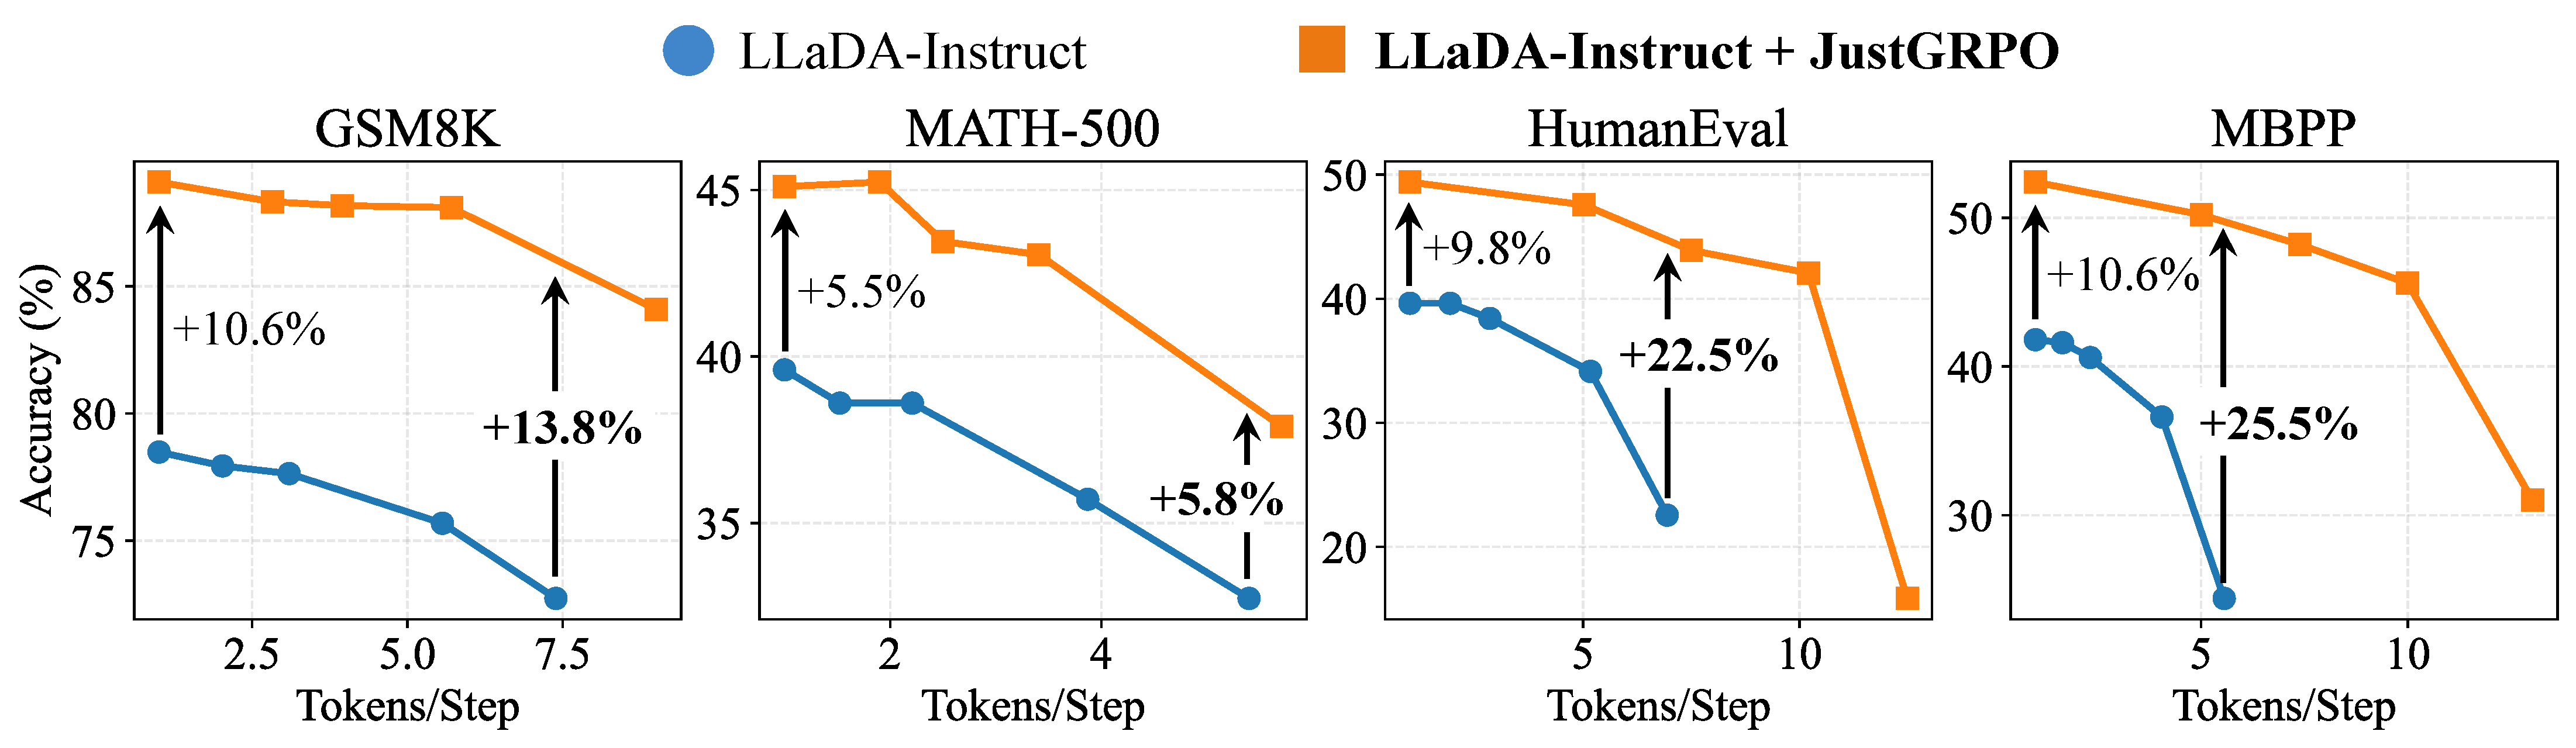
\includegraphics[width=.95\linewidth]{figures/parallel.pdf}
    \vskip -.1in
    \caption{\textbf{JustGRPO는 dLLM의 parallel decoding capability를 보존한다.}
    흥미롭게도 original instruct model과 비교하면, parallel tokens가 많을수록 accuracy gains가 더 커지는데, 이는 JustGRPO training 후 reasoning capabilities가 더 robust해졌기 때문일 가능성이 있다.
    우리는 parallel decoding을 위해 training-free EB-sampler~\cite{ben2025accelerated}를 채택한다. Generation length는 256으로 설정한다.
    }
    \label{fig:eb_sampler_comparison}
    \vskip -.05in
\end{figure}

우리는 AR training이 dLLM의 parallel decoding capabilities를 저해하는지 추가로 조사한다. Training-free Entropy Bounded (EB) Sampler~\cite{ben2025accelerated}를 사용하여 다양한 병렬성 수준(tokens per step)에서 inference performance를 평가한다.

Figure~\ref{fig:eb_sampler_comparison}는 우리 모델이 parallel decoding과 완전한 호환성을 유지하며 original LLaDA-Instruct model에 비해 speed와 accuracy 사이에서 유리한 trade-off를 보임을 보여 준다. 흥미롭게도 parallelism이 증가할수록 성능 이득은 더 두드러진다.
Baseline의 성능은 high parallel steps에서 급격히 저하되는 반면, 우리 모델은 상대적으로 더 안정적인 성능을 유지한다. 예를 들어 MBPP에서 accuracy gap은 보수적 설정(1 token/step)의 +10.6\%에서 공격적 설정($\sim$5 tokens/step)의 +25.5\%로 확대된다.
이는 특정 trajectory에 overfitting하기보다, AR formulation이 underlying model distribution을 정련하는 효과적인 training ``scaffold'' 역할을 할 수 있음을 시사한다.
이렇게 정련된 분포는 original model에 비해 parallel sampling에 내재한 approximation에 더 탄력적인 것으로 보인다.


\subsection{Training Efficiency}
\label{subsec:efficiency}

\begin{wrapfigure}{r}{0.4\textwidth}
    \centering
    \vskip -0.12in
    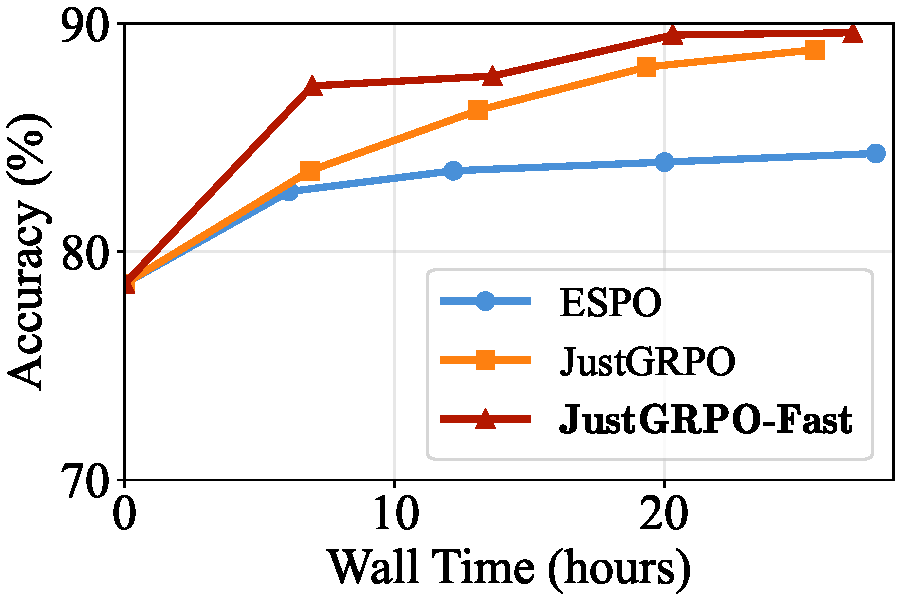
\includegraphics[width=\linewidth]{figures/gsm8k_walltime.pdf}
    \vskip -.05in
    \caption{\textbf{GSM8K에서의 training efficiency.} Iteration당 overhead가 더 큼에도, JustGRPO는 일찍 포화되는 approximation-based baseline(ESPO)보다 더 나은 accuracy/wall-time trade-off를 달성한다. JustGRPO-Fast는 가장 entropy가 높은 상위 25\% positions에서만 probability ratio $\rho_{i,k}$를 계산하여 training을 더욱 가속한다. Wall time은 16$\times$H100 GPUs에서 측정했다.}
    \label{fig:walltime_efficiency}
    \vskip -0.14in
\end{wrapfigure}
Exact GRPO를 dLLM에 적용하는 것은 구조적 trade-off를 수반한다. Autoregressive models와 달리 dLLM은 single causal forward pass가 아니라 각 position을 독립적으로 평가해야 하므로, exact likelihood를 계산하면 iteration당 추가 overhead가 발생한다. 이전 방법들~\cite{zhao2025d1,ou2025principled}은 approximation에 의존하여 이 비용을 우회했으며, 이는 비교상 exact optimization이 비실용적일 수 있음을 시사하는 듯하다. 그러나 Figure~\ref{fig:walltime_efficiency}는 그렇지 않음을 시사한다. 이러한 overhead가 있더라도 JustGRPO는 accuracy/wall-clock trade-off에서 경쟁력을 유지하며, 대표적인 approximation-based baseline(ESPO)의 peak accuracy를 비슷한 시간 안에 맞추고 계속 향상된다.

더욱이 이 overhead는 근본적인 것이 아니다. 지배적인 원인은 GRPO objective(Eq.~\ref{eq:justgrpo-loss})에서 per-position probability ratios $\rho_{i,k}$를 계산하는 데 있다. Reasoning이 sparse set of high-entropy forking tokens에 의해 조향된다는 우리의 발견(Section~\ref{sec:rethink_value_of_AO})에 동기를 얻어, 우리는 가장 entropy가 높은 상위 25\% positions에서만 $\rho_{i,k}$를 평가하여 이러한 forward evaluations의 75\%를 제거하는 JustGRPO-Fast를 도입한다.

중요하게도 per-token entropy는 rollout stage 동안 직접 기록할 수 있으므로, high-entropy positions를 식별하는 데 드는 overhead는 무시할 만하다. 경험적으로 JustGRPO-Fast는 기본 JustGRPO보다도 accuracy/wall-time trade-off를 개선하며, 기본 JustGRPO 자체도 이미 approximation-based baseline(ESPO)보다 유리하고 더 짧은 wall-clock time 안에 비슷한 accuracy에 도달한다.


